\begin{Exercise}[label={websec-cors-practs}]
	In this excercise we will see a practic demo of the CORS mechanism in action. To do so, we have adapted the website test-cors.org in order to simplify the excercise and be able to run it locally. 
	
	This test has two parts. The client is a simple page that serves a static page containing js code that can make diverse requests and runs on \url{localhost:8001}. The server is a NodeJS Express Server with CORS enabled and runs on \url{localhost:8000}. To run this demo, you have to run both the cors-server and cors-client. Then open a browser and go to \url{http://localhost:8001/} and open the browser developer tools (F12)
	
\begin{figure}[htb]
    \begin{centering}
      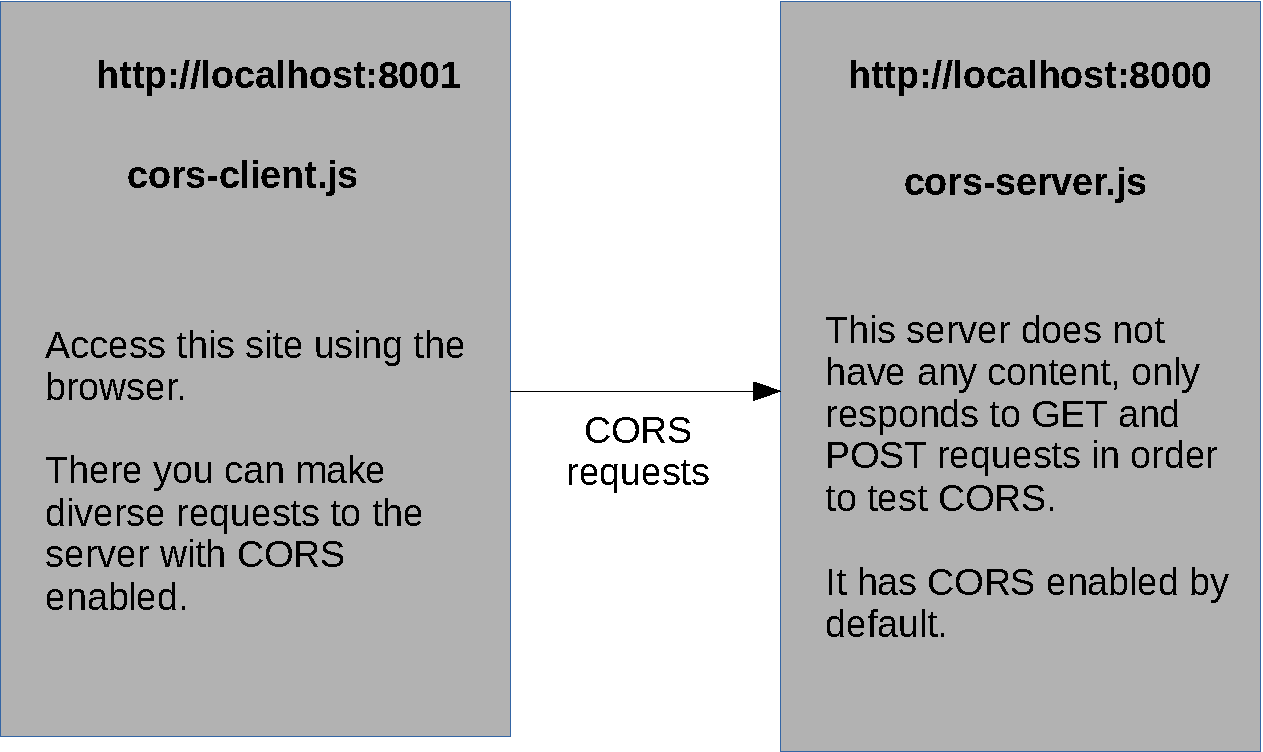
\includegraphics[width=0.7\columnwidth]{\securitydir/WebSec/figures/cors-ex}
      \par\end{centering}
    \caption{\label{fig:cors-exc} Diagram of a CORS GET request.}
 \end{figure}
  
	From this site you can choose which type of request you want to make, and observe a CORS request with and without pre-flight request. 
	You can also comment this line in the \textbf{cors-server.js} file to test what happens when CORS is not enabled.
	\begin{js}app.use(cors());\end{js} 

\end{Exercise}

\begin{Answer}[ref={websec-cors-practs}]
\end{Answer}